\documentclass[11pt]{article}
\usepackage{mathblatt}


\begin{document}
\pfheftstil
\pfheftkopf{Flaechen}{P10}
\pfrueckblick
\begin{pfaufg}{}{1.}{}
Schreib kürzer: a + a + a; a · a; 2 · a + 2 · b.
\fusshilfe{\mbox{1:~3a; a²; 2(a + b)}}
\end{pfaufg}
\begin{pfaufg}{}{2.}{}
Ergänze die Tabelle Figur | Formel.
\par\smallskip\noindent \begingroup\renewcommand{\arraystretch}{1.3}\begin{tabular}{|c|c|}\hline \textbf{Figur} & \textbf{Formel} \\ \hline A & \rule{0pt}{3ex}\hspace{1.6cm} \\ \hline A & \rule{0pt}{3ex}\hspace{1.6cm} \\ \hline A & \rule{0pt}{3ex}\hspace{1.6cm} \\ \hline A & \rule{0pt}{3ex}\hspace{1.6cm} \\ \hline A & \rule{0pt}{3ex}\hspace{1.6cm} \\ \hline\end{tabular}\endgroup\par
\fusshilfe{\mbox{2:~A = e · f : 2}}
\end{pfaufg}
\begin{pfaufg}{}{3.}{}
Zwei Halbkreise mit 5 m Durchmesser ergeben zusammen einen Kreis. Gib seinen Radius an. Ein Trapez hat unten 20 m, oben 12 m; es ist symmetrisch. Wie weit steht die untere Seite auf jeder Seite über?
\rechenraster{1}
\fusshilfe{\mbox{3:~r = 2,5 m; (20 $-$ 12) : 2 = 4 m}}
\end{pfaufg}
\pfstufekopf[sformelodertermzurfig]{Formel oder Term zur Figur}{in 3 der letzten 5 Prüfungen}
\pfgruppe{}
\begin{pfaufg}{}{4.}{}
Ein Quadrat hat den Umfang $u = 44$ cm. Kreise in der Formel $u = 4 \cdot a$ die Größe ein, die du noch nicht kennst.
\rechenraster{1}
\fusshilfe{\mbox{4:~die Seitenlänge ist gesucht}}
\end{pfaufg}
\begin{pfaufg}{}{5.}{}
Ein Garten bekommt einen Zaun. Kreuze an, ob du dafür die Fläche oder den Umfang brauchst. 
\pfkreuzzeile{Fläche}\pfkreuzzeile{Umfang}
\fusshilfe{\mbox{5:~Umfang}}
\end{pfaufg}
\begin{pfaufg}{}{6.}{}
Die Figur zeigt ein Dreieck mit der Grundseite $g$. Zeichne die Höhe zu $g$ ein und markiere den rechten Winkel.
\par\smallskip\noindent \dreieck{(0,0)}{(5,0)}{(2,3)}{}{}{g}{}{}{}\par
\rechenraster{1}
\fusshilfe{\mbox{6:~Strecke von C senkrecht auf AB}}
\end{pfaufg}
\pfgruppe{}
\begin{pfaufg}{P10 ’19}{7.}{}
Gib eine Gleichung für den Flächeninhalt A der gesamten Fläche an.
\par\smallskip\noindent 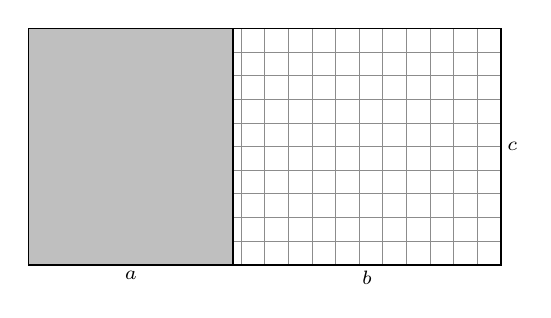
\begin{tikzpicture}[x=1.000cm,y=1.000cm,line width=0.6pt,baseline=(current bounding box.north)]\fill[black!25] (0.000,0.000) -- (2.600,0.000) -- (2.600,3.000) -- (0.000,3.000) -- cycle;\begin{scope}\clip (2.600,0.000) -- (6.000,0.000) -- (6.000,3.000) -- (2.600,3.000) -- cycle;\draw[black!45,line width=0.3pt,step=0.300] (-10,-10) grid (20,20);\end{scope}\draw (0.000,0.000) -- (6.000,0.000) -- (6.000,3.000) -- (0.000,3.000) -- cycle;\draw[] (2.600,0.000) -- (2.600,3.000);\node[font=\scriptsize,anchor=north,inner sep=2pt] at (1.300,0.000) {$a$};\node[font=\scriptsize,anchor=north,inner sep=2pt] at (4.300,0.000) {$b$};\node[font=\scriptsize,anchor=west,inner sep=2pt] at (6.000,1.500) {$c$};\end{tikzpicture}\par
\rechenraster{1}
\fusshilfe{\mbox{7:~A = (a + b) · c}}
\end{pfaufg}
\begin{pfaufg}{P10 ’22}{8.}{}
Gib eine Gleichung für den Flächeninhalt A des Dreiecks an.
\par\smallskip\noindent 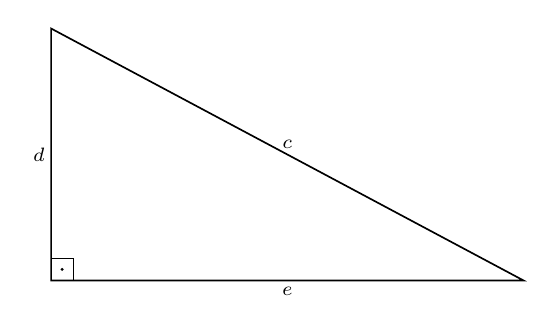
\begin{tikzpicture}[x=1.000cm,y=1.000cm,line width=0.6pt,baseline=(current bounding box.north)]\draw (0.000,0.000) -- (6.000,0.000) -- (0.000,3.200) -- cycle;\draw[line width=0.4pt] (0.280,0.000) -- (0.280,0.280) -- (0.000,0.280);\fill (0.140,0.140) circle (0.6pt);\node[font=\scriptsize,anchor=east,inner sep=2pt] at (0.000,1.600) {$d$};\node[font=\scriptsize,anchor=north,inner sep=2pt] at (3.000,0.000) {$e$};\node[font=\scriptsize,anchor=south,inner sep=2pt] at (3.000,1.600) {$c$};\end{tikzpicture}\par
\rechenraster{1}
\fusshilfe{\mbox{8:~A = d · e : 2}}
\end{pfaufg}
\pfgruppe{}
\begin{pfaufg}{P10 ’24}{9.}{}
Ein gleichseitiges Dreieck hat die Seitenlänge a. Kreuze die Formel für seinen Umfang u an:
\pfkreuzzeile{$u=a\cdot a\cdot a$}\pfkreuzzeile{$u=a^3$}\pfkreuzzeile{$u=3\cdot a$}\pfkreuzzeile{$u=\tfrac{a}{3}$}
\fusshilfe{\mbox{9:~u = 3 · a}}
\end{pfaufg}
\pfgruppe{}
\begin{pfaufg}{P10 ’14}{10.}{}
Die graue Figur ist aus gleich großen Quadraten mit der Seitenlänge a zusammengesetzt. Gib einen Term für ihren Umfang u an.
\par\smallskip\noindent \begin{tikzpicture}[line width=0.6pt,baseline=(current bounding box.north)]\draw[mbgitter,line width=0.3pt,step=0.5] (-0.5,-0.5) grid (3.0,2.0);\fill[black!30,draw=black] (0,0.5) -- (1,0.5) -- (1,0) -- (1.5,0) -- (1.5,0.5) -- (2.5,0.5) -- (2.5,1) -- (1.5,1) -- (1.5,1.5) -- (1,1.5) -- (1,1) -- (0,1) -- cycle;\node[font=\small,anchor=east] at (0,0.75) {$a$};\end{tikzpicture}\par
\rechenraster{1}
\fusshilfe{\mbox{10:~u = 16a}}
\end{pfaufg}
\pfgruppe{}
\begin{pfaufg}{P10 ’25}{11.}{}
Die Abbildung zeigt ein Rechteck. Kreuze die Gleichung an, mit der man seinen gesamten Flächeninhalt berechnet:
\pfkreuzzeile{$A=2\cdot(a+b+c)$}\pfkreuzzeile{$A=a+2\cdot a\cdot b$}\pfkreuzzeile{$A=a\cdot(b+c)$}\pfkreuzzeile{$A=a\cdot b\cdot c$}
\par\smallskip\noindent 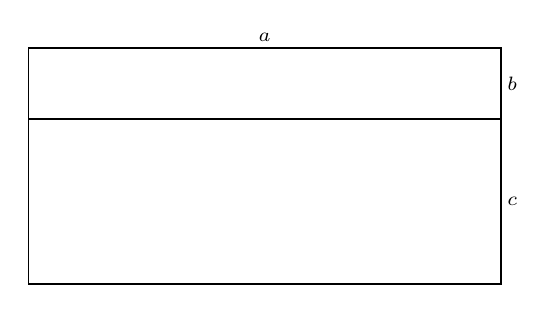
\begin{tikzpicture}[x=1.000cm,y=1.000cm,line width=0.6pt,baseline=(current bounding box.north)]\draw (0.000,0.000) -- (6.000,0.000) -- (6.000,3.000) -- (0.000,3.000) -- cycle;\draw[] (0.000,2.100) -- (6.000,2.100);\node[font=\scriptsize,anchor=south,inner sep=2pt] at (3.000,3.000) {$a$};\node[font=\scriptsize,anchor=west,inner sep=2pt] at (6.000,2.550) {$b$};\node[font=\scriptsize,anchor=west,inner sep=2pt] at (6.000,1.050) {$c$};\end{tikzpicture}\par
\fusshilfe{\mbox{11:~A = a · (b + c)}}
\end{pfaufg}
\pfstufekopf[sgrundfigurberechnen]{Grundfigur berechnen}{in 5 der letzten 5 Prüfungen}
\pfgruppe{}
\begin{pfaufg}{}{12.}{}
Du willst wissen, wie viel Farbe man für ein rundes Schild braucht. Kreuze die Formel an, die du brauchst.
\pfkreuzzeile{$u = \pi \cdot d$}\pfkreuzzeile{$A = \pi \cdot r^2$}
\fusshilfe{\mbox{12:~$\pi \cdot r^2$}}
\end{pfaufg}
\begin{pfaufg}{}{13.}{}
Die Figur zeigt ein Parallelogramm mit der Grundseite $g$. Zeichne die Höhe zu $g$ ein und markiere den rechten Winkel.
\par\smallskip\noindent \parallelogramm[seiten={$g$,,,}]{4}{2.5}{60}\par
\rechenraster{1}
\end{pfaufg}
\begin{pfaufg}{}{14.}{}
Die Figur zeigt ein Viereck. In den Formeln sind $a$ und $c$ parallele Seiten, $h$ ist die Höhe. $e$ und $f$ sind Diagonalen. Kreuze an, welche Formel zur Figur passt. 
\pfkreuzzeile{$A = a \cdot h$}\pfkreuzzeile{$A = \tfrac{a + c}{2} \cdot h$}\pfkreuzzeile{$A = \tfrac{e \cdot f}{2}$}
\par\smallskip\noindent \trapez[hoehe=h]{5}{3}{2.5}\par
\fusshilfe{\mbox{14:~$\tfrac{a + c}{2} \cdot h$}}
\end{pfaufg}
\begin{pfaufg}{}{15.}{}
Im Bild ist eine Strecke im Kreis beschriftet. Ist sie ein Radius oder ein Durchmesser? Gib auch die andere Länge an.
\par\smallskip\noindent \begin{kreis}[2] \mittelpunkt{M} \durchmesser{20}{$9$ cm} \end{kreis}\par
\par\noindent Die Strecke ist ein \leerfeld[.]  Die andere Länge: \leerfeld \par
\fusshilfe{\mbox{15:~$4{,}5$ cm}}
\end{pfaufg}
\pfgruppe{}
\begin{pfaufg}{P10 ’25}{16.}{}
Ein Drachenviereck ABCD (A links, D oben, C rechts, B unten) hat die Diagonalen AC = 50 cm und BD = 80 cm. Sie schneiden sich in F im rechten Winkel. Die Strecke DF ist 25 cm lang. Der Winkel bei D heißt $\gamma$. Ein Drachenviereck ABCD hat die Diagonalen AC = 50 cm und BD = 80 cm; sie schneiden sich im rechten Winkel. Ermittle den Flächeninhalt des Drachenvierecks.
\par\smallskip\noindent \begin{tikzpicture}[x=1.000cm,y=1.000cm,line width=0.6pt,baseline=(current bounding box.north)]\draw (0.000,1.750) -- (3.000,0.000) -- (6.000,1.750) -- (3.000,3.500) -- cycle;\draw[] (0.000,1.750) -- (3.000,1.750);\draw[] (3.000,1.750) -- (6.000,1.750);\draw[] (3.000,0.000) -- (3.000,1.750);\draw[] (3.000,1.750) -- (3.000,3.500);\draw[line width=0.4pt] (3.000,1.470) -- (3.280,1.470) -- (3.280,1.750);\fill (3.140,1.610) circle (0.6pt);\node[font=\small,inner sep=1pt] at (3.000,3.800) {$D$};\node[font=\small,inner sep=1pt] at (3.000,-0.300) {$B$};\node[font=\small,inner sep=1pt] at (-0.300,1.750) {$A$};\node[font=\small,inner sep=1pt] at (6.300,1.750) {$C$};\node[font=\small,inner sep=1pt] at (3.000,1.750) {$F$};\node[font=\scriptsize,mbgrau,anchor=north west] at ([yshift=-2pt]current bounding box.south west) {nicht maßstabsgerecht};\end{tikzpicture}\par
\rechenraster{1}
\fusshilfe{\mbox{16:~2000 cm²}}
\end{pfaufg}
\pfgruppe{}
\begin{pfaufg}{P10 ’26}{17.}{}
Ein Rechteck ist a = 3,5 cm lang und b = 1,5 cm breit. Gib seinen Umfang an.
\rechenraster{1}
\fusshilfe{\mbox{17:~10 cm}}
\end{pfaufg}
\pfgruppe{}
\begin{pfaufg}{P10 ’24}{18.}{}
Eine Firma stellt Kegel mit dem Radius r = 30 cm und der Höhe h = 80 cm her. Eine Firma stellt Kegel mit dem Radius r = 30 cm und der Höhe h = 80 cm her. Berechne den Flächeninhalt der Grundfläche eines Kegels.
\par\smallskip\noindent \begin{tikzpicture}[line width=0.6pt,baseline=(current bounding box.north)]\fill[black!15] (0,0) ellipse (1.2 and 0.36);\draw (-1.20,0.00) arc (180:360:1.20 and 0.36);\draw[dashed] (1.20,0.00) arc (0:180:1.20 and 0.36);\draw (-1.2,0) -- (0,2.4) -- (1.2,0);\node[font=\scriptsize,mbgrau,anchor=north west] at ([yshift=-2pt]current bounding box.south west) {nicht maßstabsgerecht};\end{tikzpicture}\par
\rechenraster{1}
\fusshilfe{\mbox{18:~900$\pi$ $\approx$ 2827,4 cm²}, \mbox{Tipp: $G$ = $\pi$ · 30²}}
\end{pfaufg}
\pfgruppe{}
\begin{pfaufg}{P10 ’15}{19.}{}
Gegeben ist ein Drachenviereck ABCD. Die Diagonale AC ist senkrecht (A unten, C oben), die Diagonale BD waagerecht (D links, B rechts); beide schneiden sich in E im rechten Winkel. Die Seite AD ist 4,1 cm lang. Im Dreieck ABD ist der Winkel bei A 123° und der Winkel bei B 36° groß; der Winkel bei D heißt $\delta$. Im Dreieck AED ist bei E ein rechter Winkel. Die Hypotenuse AD ist 4,1 cm lang, der Winkel bei D beträgt $\delta$ = 21°. Der Flächeninhalt des Dreiecks AED soll berechnet werden. Gib an, welche Seiten und Winkel du dazu brauchst. Schreibe die Rechenschritte in einer sinnvollen Reihenfolge auf.
\par\smallskip\noindent \begin{tikzpicture}[line width=0.6pt,baseline=(current bounding box.north)]\draw (3.40,-1.30) -- (3.40,0.00) -- (0.00,0.00) -- cycle;\node[font=\small,anchor=north] at (3.40,-1.30) {$A$};\node[font=\small,anchor=south west] at (3.40,0.00) {$E$};\node[font=\small,anchor=east] at (0,0) {$D$};\path (0.00,0.00) -- node[font=\scriptsize,below left] {4,1 cm} (3.40,-1.30);\draw[line width=0.4pt] (3.15,0.00) -- (3.15,-0.25) -- (3.40,-0.25);\draw[line width=0.4pt] (1.1,0) arc (0:-20.9:1.1);\node[font=\scriptsize,anchor=west] at (1.15,-0.2) {$\delta = 21°$};\node[font=\scriptsize,mbgrau,anchor=north west] at ([yshift=-2pt]current bounding box.south west) {nicht maßstabsgerecht};\end{tikzpicture}\par
\rechenraster{1}
\fusshilfe{\mbox{19:~21°, rechter Winkel bei E; ½ · AE · DE}}
\end{pfaufg}
\pfgruppe{}
\begin{pfaufg}{P10 ’16}{20.}{}
Beim Kugelstoßen steht man in einem Abwurfring; das ist ein Kreis mit 2,14 m Durchmesser. Ermittle den Flächeninhalt dieses Kreises.
\rechenraster{2}
\fusshilfe{\mbox{20:~1,1449$\pi$ $\approx$ 3,60 m²}}
\end{pfaufg}
\pfgruppe{}
\begin{pfaufg}{P10 ’15}{21.}{}
Mia baut das Modell einer Pyramide mit quadratischer Grundfläche: Die Grundkante ist 0,80 m lang, die Pyramide ist 0,68 m hoch. Die Seitenflächen sägt sie aus dünnem Sperrholz. Weise nach, dass sie für eine Seitenfläche etwa 0,32 m² Sperrholz braucht.
\pfzwfrage{Berechne die Höhe einer Seitenfläche mit dem Satz des Pythagoras.}
\pfzwfrage{Berechne den Flächeninhalt eines Seitendreiecks.}
\rechenraster{3}
\fusshilfe{\mbox{21:~$\approx$ 0,32 m²}}
\end{pfaufg}
\pfgruppe{}
\begin{pfaufg}{P10 ’19}{22.}{}
Auf einem Mast sitzt ein Prisma, dessen Grund- und Deckfläche gleichseitige Dreiecke mit 1,50 m Seitenlänge sind; die Höhe dieser Dreiecke beträgt 1,30 m. Das Prisma ist 1,20 m hoch. Ermittle den Flächeninhalt der Deckfläche. Durch ein Loch ist Regenwasser in das Prisma gelaufen. Zeige mit einer Rechnung, dass etwa 1,2 m³ Wasser hineinpassen. Leer wiegt das Prisma 200 kg; 1 m³ Regenwasser wiegt 1 000 kg. Berechne, wie schwer das Prisma ist, wenn ein Zehntel seines Innenraums (10 \%) voll Wasser ist.
\par\smallskip\noindent \begin{tikzpicture}[line width=0.6pt,baseline=(current bounding box.north)]\draw[fill=black!20] (0,0) -- (3,0) -- (1.5,2.6) -- cycle;\draw[dashed] (1.5,2.6) -- (1.5,0);\draw[line width=0.4pt] (1.75,0.00) -- (1.75,0.25) -- (1.50,0.25);\node[font=\scriptsize,anchor=west] at (1.5,1.2) {$h_{\text{Deckfläche}}$};\node[font=\scriptsize,mbgrau,anchor=north west] at ([yshift=-2pt]current bounding box.south west) {nicht maßstabsgerecht};\end{tikzpicture}\par
\pfzwfrage{Berechne den Flächeninhalt der Deckfläche.}
\rechenraster{5}
\fusshilfe{\mbox{22:~0,975 m²; $\approx$ 1,2 m³; $\approx$ 320 kg}}
\end{pfaufg}
\pfsteckt{steckt auch in Nr. 35 (P10 ’17); Nr. 34 (P10 ’18); Nr. 36 (P10 ’22); Nr. 38 (P10 ’23)}
\pfstufekopf[srckwrtsseiteausflche]{rückwärts: Seite aus Fläche}{in 1 der letzten 5 Prüfungen}
\pfgruppe{}
\begin{pfaufg}{P10 ’20}{23.}{}
Ein Quadrat hat den Flächeninhalt 36 cm². Gib seine Seitenlänge an.
\rechenraster{1}
\fusshilfe{\mbox{23:~6 cm}}
\end{pfaufg}
\begin{pfaufg}{P10 ’23}{24.}{}
Ein Rechteck ist 400 mm breit und hat den Flächeninhalt 42 000 mm². Gib seine Länge an.
\rechenraster{1}
\fusshilfe{\mbox{24:~105 mm}}
\end{pfaufg}
\begin{pfaufg}{P10 ’18}{25.}{}
Ein Rechteck hat den Umfang u = 26 cm; die Seite a ist 8 cm lang. Gib die Länge der Seite b an.
\par\smallskip\noindent \begin{tikzpicture}[x=1.000cm,y=1.000cm,line width=0.6pt,baseline=(current bounding box.north)]\draw (0.000,0.000) -- (6.000,0.000) -- (6.000,3.000) -- (0.000,3.000) -- cycle;\node[font=\scriptsize,anchor=north,inner sep=2pt] at (3.000,0.000) {a = 8 cm};\node[font=\scriptsize,anchor=west,inner sep=2pt] at (6.000,1.500) {$b$};\node[font=\scriptsize,mbgrau,anchor=north west] at ([yshift=-2pt]current bounding box.south west) {nicht maßstabsgerecht};\end{tikzpicture}\par
\rechenraster{2}
\fusshilfe{\mbox{25:~b = 5 cm}}
\end{pfaufg}
\pfgruppe{}
\begin{pfaufg}{P10 ’20}{26.}{}
Im Dreieck ABC ist bei C ein rechter Winkel; BC ist 12 m und AC 34 m lang. Der Punkt Q liegt auf AC. Das Dreieck QBC hat den Flächeninhalt 90 m². Berechne die Länge der Strecke QC.
\par\smallskip\noindent \begin{tikzpicture}[x=1.000cm,y=1.000cm,line width=0.6pt,baseline=(current bounding box.north)]\draw (0.000,3.500) -- (6.000,3.500) -- (0.000,0.000) -- cycle;\draw[dashed] (0.000,2.800) -- (6.000,3.500);\draw[line width=0.4pt] (0.000,3.220) -- (0.280,3.220) -- (0.280,3.500);\fill (0.140,3.360) circle (0.6pt);\node[font=\small,inner sep=1pt] at (-0.259,3.651) {$C$};\node[font=\small,inner sep=1pt] at (6.288,3.584) {$B$};\node[font=\small,inner sep=1pt] at (-0.195,-0.228) {$A$};\node[font=\small,inner sep=1pt] at (-0.292,2.868) {$Q$};\fill (0.000,2.800) circle (1.4pt);\node[font=\scriptsize,mbgrau,anchor=north west] at ([yshift=-2pt]current bounding box.south west) {nicht maßstabsgerecht};\end{tikzpicture}\par
\pfzwfrage{Stelle die Flächenformel für das Dreieck QBC auf.}
\rechenraster{2}
\fusshilfe{\mbox{26:~QC = 15 m}}
\end{pfaufg}
\pfgruppe{}
\begin{pfaufg}{P10 ’14}{27.}{}
Für ein Café wird eine Kühlvitrine in Form eines Prismas gebaut. Die Grundfläche ist ein gleichschenkliges Trapez mit den parallelen Seiten 110 cm und 80 cm, den Schenkeln 57 cm und dem Flächeninhalt 5 225 cm². Die Vitrine ist 165 cm hoch. Die Rückwand derselben Vitrine ist ein Rechteck, 110 cm breit und 165 cm hoch. Sie soll aus einer rechteckigen Platte gesägt werden, die 1,20 m breit ist und einen Flächeninhalt von 1,8 m² hat. Entscheide mit einer Rechnung, ob die Platte dafür reicht.
\par\smallskip\noindent \begin{tikzpicture}[line width=0.6pt,baseline=(current bounding box.north)]\draw (-1.50,3.70) -- (1.50,3.70) -- (1.09,2.80) -- (-1.09,2.80) -- cycle;\draw (1.50,0.90) -- (1.09,0.00) -- (-1.09,0.00) -- (-1.50,0.90);\draw[dashed] (-1.50,0.90) -- (1.50,0.90);\draw[dashed] (-1.50,0.90) -- (-1.50,3.70);\draw (1.50,0.90) -- (1.50,3.70);\draw (1.09,0.00) -- (1.09,2.80);\draw (-1.09,0.00) -- (-1.09,2.80);\path (-1.50,3.70) -- node[font=\scriptsize,above] {110} (1.50,3.70);\path (-1.09,0.00) -- node[font=\scriptsize,below] {80} (1.09,0.00);\path (1.09,2.80) -- node[font=\scriptsize,right] {57} (1.50,3.70);\path (1.09,0.00) -- node[font=\scriptsize,right] {165} (1.09,2.80);\node[font=\scriptsize,mbgrau,anchor=north west] at (-2,-0.4) {Maße in cm};\node[font=\scriptsize,mbgrau,anchor=north west] at ([yshift=-2pt]current bounding box.south west) {nicht maßstabsgerecht};\end{tikzpicture}\par
\pfzwfrage{Berechne die Länge der Platte.}
\rechenraster{2}
\fusshilfe{\mbox{27:~nein, Plattenlänge 1,5 m < 1,65 m}}
\end{pfaufg}
\pfgruppe{}
\begin{pfaufg}{P10 ’14}{\llap{\textasteriskcentered\,}28.}{}
Für ein Café wird eine Kühlvitrine in Form eines Prismas gebaut. Die Grundfläche ist ein gleichschenkliges Trapez mit den parallelen Seiten 110 cm und 80 cm, den Schenkeln 57 cm und dem Flächeninhalt 5 225 cm². Die Vitrine ist 165 cm hoch. Eine Kühlvitrine hat die Form eines Prismas. Ihre Grundfläche ist ein gleichschenkliges Trapez mit den parallelen Seiten 110 cm und 80 cm und dem Flächeninhalt 5 225 cm². Die Höhe h dieses Trapezes ist die Tiefe der Vitrine. Weise nach, dass Kuchenplatten mit 50 cm Durchmesser in die Vitrine passen.
\par\smallskip\noindent \begin{tikzpicture}[x=1.000cm,y=1.000cm,line width=0.6pt,baseline=(current bounding box.north)]\draw (0.818,0.000) -- (5.182,0.000) -- (6.000,3.000) -- (0.000,3.000) -- cycle;\draw[dashed] (0.818,3.000) -- (0.818,0.000);\draw[line width=0.4pt] (1.098,0.000) -- (1.098,0.280) -- (0.818,0.280);\fill (0.958,0.140) circle (0.6pt);\node[font=\scriptsize,anchor=north,inner sep=2pt] at (3.000,0.000) {80 cm};\node[font=\scriptsize,anchor=south,inner sep=2pt] at (3.000,3.000) {110 cm};\node[font=\scriptsize,anchor=west,inner sep=2pt] at (5.591,1.500) {57 cm};\node[font=\scriptsize,anchor=east,inner sep=2pt] at (0.818,1.500) {$h$};\node[font=\scriptsize,mbgrau,anchor=north west] at ([yshift=-2pt]current bounding box.south west) {nicht maßstabsgerecht};\end{tikzpicture}\par
\rechenraster{2}
\fusshilfe{\mbox{28:~55 cm > 50 cm $\Rightarrow$ Tiefe reicht}}
\end{pfaufg}
\pfstufekopf[sfigurerstzerlegenode]{Figur erst zerlegen oder Strecke erst berechnen}{in 3 der letzten 5 Prüfungen}
\pfgruppe{}
\begin{pfaufg}{}{29.}{}
Die Figur zeigt ein Viereck. Schreibe auf, in welche einfachen Teilflächen du es zerlegen kannst.
\par\smallskip\noindent \viereck{(0,0)}{(6,0)}{(6,3)}{(2,3)}\par
\rechenraster{1}
\fusshilfe{\mbox{29:~ein Rechteck und ein rechtwinkliges Dreieck}}
\end{pfaufg}
\begin{pfaufg}{}{30.}{}
Im Bild ist ein Teil des Kreises grau. Kreuze an, welcher Teil des Kreises das ist.
\pfkreuzzeile{$\tfrac{1}{2}$}\pfkreuzzeile{$\tfrac{1}{3}$}\pfkreuzzeile{$\tfrac{1}{4}$}
\par\smallskip\noindent \kreissektor{180}{}\par
\fusshilfe{\mbox{30:~$\tfrac{1}{2}$}}
\end{pfaufg}
\pfgruppe{}
\begin{pfaufg}{P10 ’17}{31.}{}
Familie Sommer hat einen Swimmingpool gebaut. Seine Grundfläche ist ein Rechteck, an dessen kurze Seiten je ein Halbkreis angesetzt ist. Die kurze Seite des Rechtecks ist a = 5 m lang, die lange Seite b = 10 m. Gib an, aus welchen Teilflächen die Grundfläche des Pools besteht.
\par\smallskip\noindent \begin{tikzpicture}[line width=0.6pt,baseline=(current bounding box.north)]\begin{scope}\clip (0,0) -- (3.0,0) arc (-90:90:0.9) -- (0,1.8) arc (90:270:0.9) -- cycle;\foreach \i in {-30,...,30}{\draw[line width=0.3pt] (\i*0.2-3,-3) -- ++(7,7);}\end{scope}\draw (0,0) -- (3.0,0) arc (-90:90:0.9) -- (0,1.8) arc (90:270:0.9) -- cycle;\draw[dashed] (0,0) -- (0,1.8);\node[font=\scriptsize,left,fill=white,inner sep=1pt] at (-0.9500000000000001,0.9) {$a$ = 5 m};\node[font=\scriptsize,below] at (1.5,0) {$b$ = 10 m};\node[font=\scriptsize,mbgrau,anchor=north west] at ([yshift=-2pt]current bounding box.south west) {nicht maßstabsgerecht};\end{tikzpicture}\par
\rechenraster{1}
\fusshilfe{\mbox{31:~Rechteck 10 m × 5 m und zwei Halbkreise}}
\end{pfaufg}
\pfgruppe{}
\begin{pfaufg}{P10 ’25}{32.}{}
Bestimme, wie viel Prozent der Kreisfläche grau gefärbt sind.
\par\smallskip\noindent \begin{tikzpicture}[line width=0.6pt,baseline=(current bounding box.north)]\draw (0,0) circle (1.5); \fill[black!25] (0,0) -- (90:1.5) arc (90:-55:1.5) -- cycle;\draw (0,0) -- (90:1.5); \draw (0,0) -- (-55:1.5); \fill (0,0) circle (1.3pt);\node[font=\small] at (17.5:0.9) {145°};\draw[line width=0.4pt] (0.00,0.00) ++(90:0.35) arc (90:305:0.35);\node[font=\scriptsize,fill=white,inner sep=0.5pt] at ($(0.00,0.00)+(197.5:0.6499999999999999)$) {$\alpha$};\node[font=\scriptsize,mbgrau,anchor=north west] at ([yshift=-2pt]current bounding box.south west) {nicht maßstabsgerecht};\end{tikzpicture}\par
\rechenraster{1}
\fusshilfe{\mbox{32:~$\tfrac{29}{72}$ $\approx$ 40,3 \%}}
\end{pfaufg}
\pfgruppe{}
\begin{pfaufg}{NI ’26}{33.}{}
Die Öffnung einer Taschentuchbox besteht aus einem Rechteck (13 cm × 5 cm) und zwei Halbkreisen mit 5 cm Durchmesser an den kurzen Seiten. Berechne ihren Flächeninhalt.
\par\smallskip\noindent \fbox{\parbox{0.9\linewidth}{\footnotesize Skizze: Langloch aus Rechteck 13 cm × 5 cm und zwei Halbkreisen (d = 5 cm); nicht maßstäblich}}\par
\rechenraster{2}
\fusshilfe{\mbox{33:~$\approx$ 84,63 cm²}}
\end{pfaufg}
\begin{pfaufg}{P10 ’18}{34.}{}
Ein runder Turm mit 6,4 m Durchmesser steht auf einer Rasenfläche, die 20,0 m × 12,0 m groß ist. Der Rasen um den Turm herum soll neu angelegt werden. Berechne die Fläche des neuen Rasens.
\par\smallskip\noindent \begin{tikzpicture}[line width=0.6pt,baseline=(current bounding box.north)]\draw[dotted,line width=0.9pt] (0,0) rectangle (3.6,2.4);\draw[fill=black!20] (1.8,1.2) circle (1.0);\node[font=\scriptsize,mbgrau,anchor=north west] at ([yshift=-2pt]current bounding box.south west) {nicht maßstabsgerecht};\end{tikzpicture}\par
\pfzwfrage{Berechne die Fläche des Rechtecks.}
\pfzwfrage{Berechne die Grundfläche des Turms.}
\rechenraster{3}
\fusshilfe{\mbox{34:~240 $-$ 10,24$\pi$ $\approx$ 207,83 m²}}
\end{pfaufg}
\begin{pfaufg}{P10 ’17}{35.}{}
Familie Sommer hat einen Swimmingpool gebaut. Seine Grundfläche ist ein Rechteck, an dessen kurze Seiten je ein Halbkreis angesetzt ist. Die kurze Seite des Rechtecks ist a = 5 m lang, die lange Seite b = 10 m. Berechne den Flächeninhalt der Grundfläche des Pools.
\par\smallskip\noindent \begin{tikzpicture}[line width=0.6pt,baseline=(current bounding box.north)]\begin{scope}\clip (0,0) -- (3.0,0) arc (-90:90:0.9) -- (0,1.8) arc (90:270:0.9) -- cycle;\foreach \i in {-30,...,30}{\draw[line width=0.3pt] (\i*0.2-3,-3) -- ++(7,7);}\end{scope}\draw (0,0) -- (3.0,0) arc (-90:90:0.9) -- (0,1.8) arc (90:270:0.9) -- cycle;\draw[dashed] (0,0) -- (0,1.8);\node[font=\scriptsize,left,fill=white,inner sep=1pt] at (-0.9500000000000001,0.9) {$a$ = 5 m};\node[font=\scriptsize,below] at (1.5,0) {$b$ = 10 m};\node[font=\scriptsize,mbgrau,anchor=north west] at ([yshift=-2pt]current bounding box.south west) {nicht maßstabsgerecht};\end{tikzpicture}\par
\pfzwfrage{Berechne den Flächeninhalt des Rechtecks.}
\rechenraster{3}
\fusshilfe{\mbox{35:~50 + 6,25$\pi$ $\approx$ 69,63 m²}}
\end{pfaufg}
\pfgruppe{}
\begin{pfaufg}{P10 ’22}{\llap{\textasteriskcentered\,}36.}{}
Gegeben ist ein Dreieck ABC, das nicht rechtwinklig ist. Die Höhe $h_c$ von C auf die Seite AB ist etwa 7,4 m lang; ihr Fußpunkt heißt D. Die Seite b = AC ist 14,1 m lang, der Winkel bei B ist 52° groß. Der Winkel bei C zwischen AC und der Höhe heißt $\gamma_1$. Im Dreieck ABC ist die Höhe $h_c$ $\approx$ 7,4 m; ihr Fußpunkt D liegt auf AB. Der Winkel bei B beträgt 52°. Gegeben: AD $\approx$ 12,0 m. Ermittle den Flächeninhalt des Dreiecks ABC.
\par\smallskip\noindent \begin{tikzpicture}[x=1.000cm,y=1.000cm,line width=0.6pt,baseline=(current bounding box.north)]\draw (0.000,0.000) -- (6.000,0.000) -- (3.000,3.500) -- cycle;\draw[dashed] (3.000,3.500) -- (3.000,0.000);\draw[line width=0.4pt] (3.000,0.280) -- (2.720,0.280) -- (2.720,0.000);\fill (2.860,0.140) circle (0.6pt);\draw[line width=0.4pt] (5.727,0.319) arc (130.60:180.00:0.420);\node[font=\scriptsize,inner sep=0.5pt,fill=white] at (5.164,0.384) {52°};\node[font=\scriptsize,anchor=west,inner sep=2pt] at (3.000,1.750) {$h_c$};\node[font=\scriptsize,anchor=east,inner sep=2pt] at (1.500,1.750) {b = 14,1 m};\node[font=\small,inner sep=1pt] at (-0.280,-0.109) {$A$};\node[font=\small,inner sep=1pt] at (6.280,-0.109) {$B$};\node[font=\small,inner sep=1pt] at (3.000,3.800) {$C$};\node[font=\small,inner sep=1pt] at (3.000,-0.300) {$D$};\node[font=\scriptsize,mbgrau,anchor=north west] at ([yshift=-2pt]current bounding box.south west) {nicht maßstabsgerecht};\end{tikzpicture}\par
\rechenraster{3}
\fusshilfe{\mbox{36:~A = 3,7 · (√144,05 + 7,4 : tan 52°) $\approx$ 65,8 m²}}
\end{pfaufg}

\pfstufekopf[santeilinprozentversc]{Anteil in Prozent (Verschnitt)}{in 1 der letzten 5 Prüfungen}
\pfgruppe{}
\begin{pfaufg}{NI ’22}{37.}{}
Simone schneidet eine runde Tischdecke mit 115 cm Durchmesser aus einem Stoffrechteck von 15 000 cm². Der Rest ist Verschnitt. Berechne den Verschnitt in Prozent.
\rechenraster{3}
\fusshilfe{\mbox{37:~$\approx$ 10 386,89 cm²; $\approx$ 30,75 \%}}
\end{pfaufg}
\pfgruppe{}
\begin{pfaufg}{P10 ’23}{\llap{\textasteriskcentered\,}38.}{}
Eine Konservendose hat die Form eines Zylinders mit dem Radius 4 cm und der Höhe 8 cm. Für Konservendosen werden kreisrunde Deckel mit dem Radius 4 cm aus Blechstreifen ausgestanzt, die 8 cm breit und 1 m lang sind. Aus jedem Streifen sollen möglichst viele Deckel entstehen. Der Abfall darf höchstens 25 \% eines Streifens ausmachen. Überprüfe rechnerisch, ob diese Vorgabe eingehalten wird.
\pfzwfrage{Berechne, wie viele Deckel aus einem Streifen ausgestanzt werden können.}
\pfzwfrage{Berechne die Fläche aller Deckel eines Streifens.}
\pfzwfrage{Berechne die Fläche eines Streifens.}
\rechenraster{4}
\fusshilfe{\mbox{38:~$\approx$ 24,6 \% $\le$ 25 \%}}
\end{pfaufg}
\pfpruefstein{P10 ’23}
\begin{pfaufg}{}{}{}
Gegeben ist ein Trapez mit den parallelen Seiten 25,80 m (unten) und 15,00 m (oben). Es ist 8,00 m hoch. Die beiden Winkel an der unteren Seite sind je 56° groß.
\par\smallskip\noindent \begin{tikzpicture}[x=1.000cm,y=1.000cm,line width=0.6pt,baseline=(current bounding box.north)]\draw (0.000,0.000) -- (6.000,0.000) -- (4.744,1.860) -- (1.256,1.860) -- cycle;\draw[dashed] (1.256,1.860) -- (1.256,0.000);\draw[line width=0.4pt] (1.536,0.000) -- (1.536,0.280) -- (1.256,0.280);\fill (1.396,0.140) circle (0.6pt);\draw[line width=0.4pt] (0.420,0.000) arc (0.00:55.98:0.420);\node[font=\scriptsize,inner sep=0.5pt,fill=white] at (0.812,0.432) {56°};\draw[line width=0.4pt] (5.765,0.348) arc (124.02:180.00:0.420);\node[font=\scriptsize,inner sep=0.5pt,fill=white] at (5.188,0.432) {56°};\draw[line width=0.4pt] (4.324,1.860) arc (180.00:304.02:0.420);\node[font=\scriptsize,inner sep=0.5pt,fill=white] at (4.397,1.207) {$\gamma$};\node[font=\scriptsize,anchor=north,inner sep=2pt] at (3.000,0.000) {25,80 m};\node[font=\scriptsize,anchor=south,inner sep=2pt] at (3.000,1.860) {15,00 m};\node[font=\scriptsize,anchor=east,inner sep=2pt] at (1.256,0.930) {8,00 m};\node[font=\scriptsize,mbgrau,anchor=north west] at ([yshift=-2pt]current bounding box.south west) {nicht maßstabsgerecht};\end{tikzpicture}\par
\end{pfaufg}
\begin{pfaufg}{}{a)}{1 BE}
Ein Trapez hat die parallelen Seiten 25,80 m (unten) und 15,00 m (oben) und ist 8,00 m hoch. Die beiden Winkel an der unteren Seite sind je 56° groß. Gib die Größe des Winkels $\gamma$ oben rechts an.
\rechenplatz{3}
\fusshilfe{\mbox{Prüfstein a):~$\gamma$ = 124°}}
\end{pfaufg}
\begin{pfaufg}{}{b)}{2 BE}
Berechne den Flächeninhalt des Trapezes.
\rechenplatz{3}
\fusshilfe{\mbox{Prüfstein b):~A = 163,2 m²}}
\end{pfaufg}
\begin{pfaufg}{}{*c)}{3 BE}
Berechne den Umfang des Trapezes.
\rechenplatz{3}
\fusshilfe{\mbox{Prüfstein c):~U = 40,8 + 16 : sin 56° $\approx$ 60,1 m}}
\end{pfaufg}
\end{document}